\documentclass[12pt,aspectratio=169]{beamer}
\input{../mybeamer}

\title{Class 5: Circuit Analysis, Part 1}
\subtitle{AP Physics 2}
\input{../me}
\input{../mycommands}


\begin{document}

\begin{frame}
  \maketitle
\end{frame}


\section{Circuits}

\begin{frame}{Basic DC Circuit}
  \begin{columns}
    \column{.3\textwidth}
    \centering
    \begin{tikzpicture}[scale=1.8,american voltages,thick]
      \draw (0,0) to[battery,l=$\mathcal E$] (0,1.5)--(1.5,1.5) to[R=$R$]
      (1.5,0)--(0,0);
    \end{tikzpicture}
    
    \column{.7\textwidth}
    A basic circuits consists of:
    \begin{itemize}
    \item An energy source:
      \begin{itemize}
      \item Examples: battery, generator or capacitor
      \item Creates a voltage gain, called the \textbf{electromotive force}, or
        \emph{emf} ($\mathcal E$)
      \end{itemize}
    \item Loads:
      \begin{itemize}
        \item resistors, motor, LEDs
      \end{itemize}
    \item Connecting wires:
      \begin{itemize}
      \item Assume to have negligible resistance
      \end{itemize}
    \end{itemize}
  \end{columns}
\end{frame}



\section{Electric Current}

\begin{frame}{Electric Current}
  In an electric circuit, a large number of charge ``carriers'' are pushed
  along by a small electrostatic force in a conductive material, creating an
  \textbf{electric current}. We can imagine positive charges moving from the
  positive terminal towards the negative terminal.
  \begin{center}
    \begin{tikzpicture}[scale=.85,thick]
      \fill[magenta!10] rectangle (7,3);
      \draw[very thick] (0,0)--(7,0);
      \draw[very thick] (0,3)--(7,3);
      
      \draw[fill=cyan!20] (1,.5) circle(.25) node{$+$};
      \draw[axes] (1.25,.5)--(1.75,.5);

      \draw[fill=cyan!20] (3,.75) circle(.25) node{$+$};
      \draw[axes] (3.25,.75)--(3.75,.75);

      \draw[fill=cyan!20] (6,1.75) circle(.25) node{$+$};
      \draw[axes] (6.25,1.75)--(6.75,1.75);

      \draw[fill=cyan!20] (5,2.5) circle(.25) node{$+$};
      \draw[axes] (5.25,2.5)--(5.75,2.5);

      \draw[fill=cyan!20] (4,1.75) circle(.25) node{$+$};
      \draw[axes] (4.25,1.75)--(4.75,1.75);

      \draw[fill=cyan!20] (5.25,1) circle(.25) node{$+$};
      \draw[axes] (5.5,1)--(6,1);

      \draw[fill=cyan!20] (2,1.5) circle(.25) node{$+$};
      \draw[axes] (2.25,1.5)--(2.75,1.5);

      \draw[fill=cyan!20] (.5,2.5) circle(.25) node{$+$};
      \draw[axes] (.75,2.5)--(1.25,2.5);

      \draw[fill=cyan!20] (2.5,2.25) circle(.25) node{$+$};
      \draw[axes] (2.75,2.25)--(3.25,2.25);

      \node at (0,1.5)[left] {\huge$+$};
      \node at (7,1.5)[right]{\huge$-$};
    \end{tikzpicture}
  \end{center}
  In a metal conductor, \textbf{charge carriers} are freely-moving electrons.
  But in other applications protons or ions can also generate a current.
\end{frame}



\begin{frame}{Electrical Current}
  The average \textbf{electrical current} $I$ through conductor is the amount
  of charges $Q$ that passes through a point during a finite time interval
  $\Delta t$:

  \eq{-.1in}{
    \boxed{I=\frac Q{\Delta t}}
  }

  Generally, the current through a conductor is a function of time ($I=I(t)$),
  and $+/-$ signs may be used to indicate direction of the current.
\end{frame}



\begin{frame}{Direct and Alternating Current}
  In a \textbf{direct current} (\textbf{DC}), the flow of charges is always in
  the same direction, but the current itself does not have to be constant in
  time. Below are all examples of direct currents.
  
  \begin{center}
    \begin{tikzpicture}[scale=.7]
      \draw[red,ultra thick] (0,3)--(4,3);
      \draw[axes] (0,0)--(4,0) node[right]{$t$};
      \draw[axes] (0,0)--(0,4) node[above]{$I$};
    \end{tikzpicture}
    \begin{tikzpicture}[scale=.7]
      \draw[smooth,samples=20,domain=0:3.5,functions]
      plot(\x,{3*(exp(-.8*\x))});
      \draw[axes] (0,0)--(4,0) node[right]{$t$};
      \draw[axes] (0,0)--(0,4) node[above]{$I$};
    \end{tikzpicture}
    \begin{tikzpicture}[scale=.7]
      \draw[axes] (0,0)--(4,0) node[right]{$t$};
      \draw[axes] (0,0)--(0,4) node[above]{$I$};
      \draw[smooth,samples=20,domain=0:3.5,functions]
      plot(\x,{sin(120*\x)+2});
    \end{tikzpicture}
  \end{center}
\end{frame}



\begin{frame}{Direct and Alternating Current}
  In an \textbf{alternating current} (\textbf{AC}), the flow of charges changes
  in direction, \emph{usually} as a sinusoidal function of time.
  \begin{center}
    \begin{tikzpicture}[scale=.6]
      \draw[smooth,samples=50,domain=0:4,functions] plot(\x,{1.5*sin(150*\x)});
      \draw[axes] (0,0)--(5,0) node[right]{$t$};
      \draw[axes] (0,-2.5)--(0,2.5) node[above]{$I$};
    \end{tikzpicture}
    \begin{tikzpicture}[scale=.6]
      \draw[smooth,samples=50,domain=0:4,functions] plot(\x,{1.5*sin(150*\x)});
      \draw[axes] (0,0)--(5,0) node[right]{$t$};
      \draw[axes] (0,-2.5)--(0,2.5) node[above]{$V$};
    \end{tikzpicture}
  \end{center}
  The power outlet in North America are all AC, with a maximum voltage of
  \SI{120}\volt, and a frequency of \SI{60}\hertz.
\end{frame}



%\begin{frame}{Current Through the Conductor}
%  The expression for electric current can be expanded this way:
%  
%  \eq{-.1in}{
%    I=\frac Q{\Delta t}=\left(\frac QV\right)\frac V{\Delta t}
%    =\left[ne\right]\left[Av_d\right]
%  }
%  where
%  \begin{itemize}
%  \item $Q/V$ is the \emph{amount of charges per volume}, which is also the
%    \textbf{charge carrier density} (number of charge carriers per volume) $n$
%    times the \textbf{elementary charge} $e$
%  \item $V/t$ is the rate the volume of charges moves through the
%    conductor, give by the cross-section area of the conductor $A$ times the
%    \textbf{drift velocity} $v_d$ of the charge carrier
%  \end{itemize}
%\end{frame}
%
%
%
%\begin{frame}{Charge Carrier Density}
%  Calculating the charge carrier density in a \emph{metal} conductor involves
%  some physical information about the metal:
%  \begin{enumerate}
%  \item Divide the metal's density $\rho$ by its molar mass $M$ to find the
%    \emph{number of moles of atoms per unit volume}
%  \item Multiply by Avogadro's number $N_A=\SI{6.0221e23}{\per mol}$ to find
%    \emph{number of atoms per unit volume}
%  \item Multiply by the number of free electrons per atom $k$ for that
%    particular metal
%  \end{enumerate}
%\end{frame}
%
%
%
%\begin{frame}{Charge Carrier Density}
%  Collecting all the terms from the last slide, we have:
%  
%  \eq{-.1in}{
%    \boxed{n=\frac{\rho kN_A}M}
%  }
%  \begin{center}
%    \begin{tabular}{l|c|c}
%      \rowcolor{pink}
%      \textbf{Quantity} & \textbf{Symbol} & \textbf{SI Unit} \\ \hline
%      Charge carrier density   & $n$    & \si{\per\metre\cubed} \\
%      Density of material      & $\rho$ & \si{\kilo\gram\per\metre\cubed} \\
%      Free electrons per atom  & $k$    & \\
%      Avogadro's number        & $N_A$  & \si{\per\mol}\\
%      Molar mass               & $M$    & \si{\kilo\gram\per\mol}
%    \end{tabular}
%  \end{center}
%  For copper, $M=\SI{63.54e-3}{\kilo\gram\per\mol}$,
%  $\rho=\SI{8.96e3}{\kilo\gram\per\metre\cubed}$, $k=1$ and therefore
%  $n=\SI{8.5e28}{\per\metre\cubed}$.
%\end{frame}
%
%
%
%\begin{frame}{Current}
%  Another alternate description of the electric current is to express it in
%  terms of the current density $J$, with a unit of of \emph{amp\`{e}re per
%  meters squared} (\si{\ampere\per\meter\squared}).
%  
%  \eq{-.1in}{
%    \boxed{I=JA}
%  }
%
%  It is obvious from the previous expression that the current density is the
%  product of the charge carrier density, elementary charge, and the drift
%  velocity:
%
%  \eq{-.1in}{
%    \boxed{J=nev_d}
%  }
%\end{frame}



\begin{frame}{Conventional Current vs.\ Electron Flow}
  We have \emph{assumed} that the charge carriers are positively charged, which
  means that the current flows from high electric potential to low potential
  (i.e.\ from cathode to anode).
  \begin{center}
    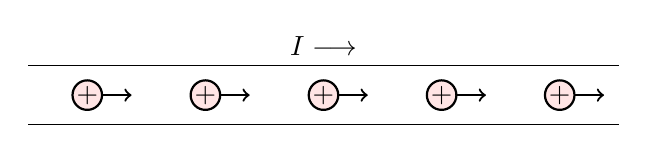
\begin{tikzpicture}[scale=.75]
      \draw (0,0)--(10,0);
      \draw (0,1)--(10,1) node[midway,above]{$I\longrightarrow$};
      \foreach \x in {1,3,...,9}{
        \draw[thick,fill=pink!40] (\x,.5) circle (.25) node{$+$};
        \draw[thick,->] (\x+.25,.5)--(\x+.75,.5);
      }
    \end{tikzpicture}
  \end{center}
  In a conducting wire, instead of positive charges flowing in one direction,
  we have, in fact, electrons (negative charges) flowing in the opposite
  direction, called the \textbf{electron flow}, or \textbf{electron current}:
  \begin{center}
    \begin{tikzpicture}[scale=.75]
      \draw (0,0)--(10,0);
      \draw (0,1)--(10,1) node[midway,above]{$I\longrightarrow$};
      \foreach \x in {1,3,...,9}{
        \draw[thick,fill=blue!40!gray!20] (\x,.5) circle (.25) node{$-$};
        \draw[axes] (\x-.25,.5)--(\x-.75,.5);
      }
    \end{tikzpicture}
  \end{center}
  For circuit analysis, we use the conventional current for simplicity.
\end{frame}



\begin{frame}{Electric Field Inside the Wire}
  Inside the wire, there is a weak electric field, which exerts a force on the
  free electrons as they move in the wire
  \begin{itemize}
  \item As the charges move through a conductor, they lose potential energy
  \item Unlike a falling object which converts gravitational potential energy
    to kinetic energy, in a circuit, the energy is 
    \begin{itemize}
    \item converted into radiative heat or light through the resistance of the
      wire, or
    \item converted into kinetic energy of a motor shaft
    \end{itemize}
  \end{itemize}
\end{frame}



\section{Resistors}


\begin{frame}{Circuit Diagrams: Loads}
  Loads are devices that transforms the electrical energy in the circuit into
  other forms of energy. Examples include:
  \begin{center}
    \begin{circuitikz}[american voltages]
      \draw[thick] (0,0) to[R,l=Resistor,o-o] (2,0);
      \draw[thick] (3,0) to[bulb,l=Light Bulb,o-o] (5,0);
      \draw[thick] (6,0) to[lamp,l=Lamp,o-o] (8,0);
      \draw[thick] (9,0) to[short,o-o] (11,0);
      \draw[very thick,fill=white] (9.35,-.2) rectangle (10.65,.2);
      \draw[very thick,fill=white] (10,0) circle (14pt) node{M};
      \node at (10,.8) {Motor};
    \end{circuitikz}
  \end{center}
  \begin{itemize}
    \item Resistors, light bulbs and other lamps transform electrical energy
      into heat, light and other forms of
      \textbf{electromagnetic radiation}\footnote{Also known as
      \textbf{electromagnetic waves}, or \textbf{EM waves}. They include radio
      waves, microwaves, infrared radiation, visible light, ultraviolet (UV)
      radiation, x-ray and gamma rays}
    \item A motor converts electrical energy into kinetic energy of the motor
      shaft and whatever objects are connected to it through an interaction
      with a magnetic field inside the motor
  \end{itemize}
  \vspace{.2in}
  %Other things to have in a circuit (switches, fuse)  
\end{frame}



\begin{frame}{Ohm's Law}
  The electric potential difference $V$ across a resistor equals the product of
  the current $I$ through the load and the resistance $R$:

  \eq{-.2in}{
    \boxed{V=IR}
  }
  \begin{center}
    \begin{tabular}{l|c|c}
      \rowcolor{pink}
      \textbf{Quantity} & \textbf{Symbol} & \textbf{SI Unit} \\ \hline
      Potential difference & $V$    & \si\volt \\
      Current              & $I$    & \si\ampere \\
      Resistance           & $R$    & \si\ohm
    \end{tabular}
  \end{center}
  A load is considered ``ohmic'' if it obeys Ohm's law. Note that Ohm's law
  is not a fundamental law in physics.
\end{frame}



\begin{frame}{Resistance of a Conductor}
  The resistance of a conductor is proportional to the resistivity $\rho$ and
  its length $L$, and inversely proportional to the cross-sectional area $A$:

  \eq{-.1in}{
    \boxed{
      R=\rho\frac LA
    }
  }
  \begin{center}
    \begin{tabular}{l|c|c}
      \rowcolor{pink}
      \textbf{Quantity} & \textbf{Symbol} & \textbf{SI Unit} \\ \hline
      Resistance           & $R$    & \si\ohm \\
      Resistivity          & $\rho$ & \si{\ohm\metre}\\
      Length of conductor  & $L$    & \si\metre \\
      Cross-sectional area & $A$    & \si{\metre\squared}
    \end{tabular}
  \end{center}
  The resistivity $\rho$ is determined by the material.
\end{frame}



%\begin{frame}{Resistivity}
%  The resistivity of a material is the ratio between strength of the electric
%  field $E$ inside the material and the current density $J$:
%
%  \eq{-.1in}{
%    \boxed{\rho=\frac EJ}
%  }
%  \begin{itemize}
%  \item Conductor: the electrons are free to move, therefore the electric
%    field tend to be very small, and the resistivity is low.
%  \item Insulators and dielectric: electrons cannot move easily (dielectric:
%    they can only polarize themselves) the electric field are generally
%    strong, and the resistivity is higher.
%  \end{itemize}
%\end{frame}



\begin{frame}{Resistance of a Conductor}

  \eq{.0in}{
    \boxed{R=\rho\frac LA}
  }
  
  \begin{columns}[T]
    \column{.5\textwidth}
    \centering
    \begin{tabular}{c|c|c}
      \rowcolor{blue!50}
               {\color{white}Gauge} & 
               {\color{white}Diameter} & 
               {\color{white}$R/L$} \\
               \rowcolor{blue!50}
        & {\color{white}(\si{\milli\metre})} & 
                        {\color{white}(\SI{e-3}{\ohm\per\metre})}\\ \hline
                        0  & \num{9.35} & \num{0.31} \\
                        10 & \num{2.59} & \num{2.20} \\
                        14 & \num{1.63} & \num{8.54} \\
                        18 & \num{1.02} & \num{21.90} \\
                        22 & \num{0.64} & \num{51.70} \\
    \end{tabular}
    
    \column{.5\textwidth}
    \centering
    \begin{tabular}{c|c}
      \rowcolor{blue!50}
               {\color{white} Material} & 
               {\color{white} Resistivity $\rho$ (\si{\ohm\metre})}\\ \hline
               silver    & \num{1.6e-8} \\
               copper    & \num{1.7e-8} \\
               aluminum  & \num{2.7e-8} \\
               tungsten  & \num{5.6e-8} \\
               Nichrome  & \num{100e-8} \\
               carbon    & \num{3500e-8}\\
               germanium & \num{.46} \\
               glass     & \num{e10} to \num{e14}\\
    \end{tabular}
  \end{columns}
\end{frame}



\begin{frame}{Ohmic vs.\ Non-Ohmic Devices}
  In an \textbf{ohmic device} such as a resistor, the relationship between
  voltage across the device and the current through the device is linear:
  \begin{center}
    \begin{tikzpicture}[scale=.7]
      \draw[functions] (0,0)--(2.5,2.5) node[right]{$\text{slope}=R$};
      \draw[axes] (0,0)--(3,0) node[right]{$I$};
      \draw[axes] (0,0)--(0,3) node[right]{$V$};
    \end{tikzpicture}
    \hspace{.15in}
    \begin{tikzpicture}[scale=.7]
      \draw[functions] (0,0)--(2.5,2.5)
      node[right]{$\text{slope}=\dfrac1R$};
      \draw[axes] (0,0)--(3,0) node[right]{$V$};
      \draw[axes] (0,0)--(0,3) node[right]{$I$};
    \end{tikzpicture}
  \end{center}
\end{frame}



\begin{frame}{Ohmic vs.\ Non-Ohmic Devices}
  Loads that are \textbf{non-ohmic} do not obey Ohm's law; the relationship
  between voltage and current is \emph{not} linear. For example, diodes (e.g.\
  your TV's LED screen) are non-ohmic.
  \begin{center}
    \begin{tikzpicture}[scale=.7]
      \draw[axes] (0,0)--(3,0) node[right]{$V$};
      \draw[axes] (0,0)--(0,3) node[right]{$I$};
      \draw[functions,domain=0:2.45,smooth] plot(\x,.0008*\x^9);
    \end{tikzpicture}
  \end{center}
\end{frame}



\begin{frame}{Power Dissipated by a Load}
  Average power $P$ is the rate at which work $W$ is done, and from
  electrostatics, the change in electric potential energy $\Delta E_q$ is
  proportional to the amount of charge $q$ and the voltage $V$. This gives a
  very simple expression for power through a resistor:
  
  \eq{-.1in}{
    P=\frac W{\Delta t}=\frac{\Delta (qV)}{\Delta t}
    =\left(\frac{\Delta q}{\Delta t}\right)V
    \;\rightarrow\;\boxed{P=IV}
  }
  \begin{center}
    \begin{tabular}{l|c|c}
      \rowcolor{pink}
      \textbf{Quantity} & \textbf{Symbol} & \textbf{SI Unit} \\ \hline
      Power through a load    & $P$ & \si\watt \\
      Current through a load  & $I$ & \si\ampere \\
      Voltage across the load & $V$ & \si\volt
    \end{tabular}
  \end{center}
  This relationship applies regardless of whether the loads are ohmic or not
\end{frame}



\begin{frame}{Other Equations for Power}
  Combining Ohm's law ($V=IR$) with power equation, we get two additional
  expressions for power through a resistor:

  \eq{-.1in}{
    \boxed{P=\frac{V^2}R}\quad\quad\boxed{P=I^2R}
  }
  \begin{center}
    \begin{tabular}{l|c|c}
      \rowcolor{pink}
      \textbf{Quantity} & \textbf{Symbol} & \textbf{SI Unit} \\ \hline
      Power      & $P$ & \si\watt \\
      Voltage    & $V$ & \si\volt \\
      Resistance & $R$ & \si\ohm  \\
      Current    & $I$ & \si\ampere
    \end{tabular}
  \end{center}
  Not surprisingly, these equations will only apply to ohmic devices.
\end{frame}


\section{Other Circuit Devices}

\begin{frame}{Other Circuit Devices}
  An energy sources may include:
  \begin{center}
    \begin{tikzpicture}[american voltages,thick]
      \draw (-3,0) to[battery1,l=Voltaic Cell,o-o] (-1,0);
      \draw (0,0) to[battery, l=Battery,o-o] (2,0);
      \draw (3,0) to[pvsource,l=Solar Panel,o-o] (5,0);
      %\draw (3,0) to[C,l=Capacitor,o-o] (5,0);
      \draw (6,0) to[american voltage source,l=DC Voltage,o-o] (8,0);
      \draw (9,0) to[sinusoidal voltage source,l=AC Voltage,o-o] (11,0);
    \end{tikzpicture}
  \end{center}
  A \textbf{capacitor} also acts as a energy source. When a capacitor is
  charged---with charge $+Q$ on one plate, and $-Q$ on the other, a voltage
  is generated, according to the equation $V=Q/C$ (studied in Class 5).
  \begin{center}
    \begin{tikzpicture}[thick]
      \draw (3,0) to[C,l=Capacitor,o-o] (5,0);
    \end{tikzpicture}
  \end{center}
  Circuits with both resistors and capacitors will be studied next class.
\end{frame}




\begin{frame}{Other Circuit Devices}
  There are also other circuit devices that are not strictly necessary, but
  are very important/useful to ensure the reliable operation of an electrical
  circuit. For examples:
  \begin{columns}[T]
    \column{.3\textwidth}
    \begin{center}
      \vspace{.15in}
      \begin{tikzpicture}[thick,scale=1.2]
        \draw (0,0) to[fuse,l=Fuse,o-o] (2,0);
      \end{tikzpicture}
    \end{center}
    A \textbf{fuse} will break (stopping current from flowing) when the
    current through it exceeds its rating.

    \column{.4\textwidth}
    \begin{center}
      \begin{tikzpicture}[thick]
        \draw (0,0) to[short,o-] (.7,0) to[short,-*]
        +({.6*cos(40)},{.6*sin(40)});
        \draw (1.3,0) to[short,*-o] (2,0);
        \node at (1,.8){Switch};
      \end{tikzpicture}
    \end{center}
    \vspace{.03in}A switch allows the circuit to be manually turned on or off.
    (In the example above, the switch is open and no current flows through it.)
  \end{columns}
\end{frame}


\begin{frame}{Measuring Devices}
  \begin{columns}[T]
    \column{.3\textwidth}
    \begin{tikzpicture}[scale=1.5]
      \draw[thick] (.2,0) to[R,l=$R$] (2.8,0);
      \draw[thick] (.7,0) to[short,*-](.7,-.8)--(2.3,-.8) to[short,-*] (2.3,0);
      \draw[very thick,fill=black!2] (1.5,-.8) circle (.3) node{V};
    \end{tikzpicture}
    
    A \textbf{voltmeter} is placed in \emph{parallel} with a load to measure
    the voltage across it. An ideal voltmeter has infinite resistance
    ($R=\infty$) and no current through it ($I=0$).

    \column{.3\textwidth}
    \begin{tikzpicture}[scale=1.5]
      \draw[thick] (0,0) to[short] (1,0) to[R,l=$R$] (2.8,0);
      \draw[very thick,fill=black!2] (.7,0) circle (.3) node{A};
    \end{tikzpicture}
    
    \vspace{.47in}An \textbf{ammeter} is placed in \emph{series} with a load to
    measure the current through it. An ideal ammeter has zero resistance
    ($R=0$), thus it does not alter the flow of current in the circuilt

    \column{.3\textwidth}
    \begin{tikzpicture}[scale=1.5]
      \draw[thick] (0,0) to[R,l=$R$] (3,0);
      \draw[thick] (.7,0) to[short,*-] (.7,-.8)--(2.3,-.8) to[short,-*](2.3,0);
      \draw[very thick,fill=black!2] (1.5,-.8) circle (.3) node{$\Omega$};
    \end{tikzpicture}    
    
    An \textbf{ohmmeter} is placed in \emph{parallel} with a load to measure
    the resistance across the load.
  \end{columns}
\end{frame}



\begin{frame}{Digital Multi-Meter}
  \begin{columns}
    \column{.3\textwidth}
    \pic1{voltmeter}

    \column{.7\textwidth}
    \begin{itemize}
    \item Voltmeters, ammeters and ohmmeters operate on the same principle
      using magnetic effects inside the device, called a \textbf{galvanometer}.
    \item Modern voltmeters are usually part of a \textbf{multi-meter} that
      also operates as an ammeter and ohmmeter.
    \end{itemize}
  \end{columns}
\end{frame}


\section{Kirchhoff's Laws}

\begin{frame}{Kichhoff's Junction Law}
  In the \textbf{junction law}, also known as the \textbf{current law}, the
  electrical current that flows into any junction in a circuit must
  be equal to the current which flows out.

  \vspace{.05in}
  \begin{columns}[T]
    \column{.3\textwidth}
    \centering
    \begin{tikzpicture}[scale=1.2]
      \draw[thick] (1,1) to[short,o-*] (1,0)--(0,0)--(0,-.7) to[R] (0,-2);
      \draw[thick] (1,-2) to[C] (1,-.7)--(1,0)--(2,0)--(2,-.7) to[L] (2,-2);
      \begin{scope}[ultra thick,red,->]
        \draw (1,.9)--(1,.1) node[midway,right]{$I$};
        \draw (.9,0)--(.1,0) node[midway,above]{$I_1$};
        \draw (1,-.1)--(1,-.9) node[midway,right]{$I_2$};
        \draw (1.1,0)--(1.9,0) node[midway,above]{$I_3$};
      \end{scope}
    \end{tikzpicture}
    
    \column{.7\textwidth}
    In the example, there are 4 paths to the junction at the centre, with $I$
    flowing into the junction, and $I_1$, $I_2$, $I_3$ flowing out, then the
    junction law says that

    \eq{-.15in}{
      I=I_1+I_2+I_3
    }

    \vspace{-.18in}regardless of what circuit devices those paths are connected
    to. In the example, a resistor, a capacitor and an inductor (not part of AP
    Physics 2) are joined at the junction.
  \end{columns}
  \vspace{.13in}It means that there must be accumulation of charges
  anywhere in the circuit.
\end{frame}



\begin{frame}{Kichhoff's Voltage Law}
  In the \textbf{voltage law}, the voltage changes around any closed loop in
  the circuit must sum to zero, no matter what path you take through an
  electrical circuit.

  \vspace{.1in}
  \begin{columns}
    \column{.45\textwidth}
    \begin{tikzpicture}[scale=1.55,american voltages,thick]
      \draw (0,0) to[battery,l=$\mathcal E$] (0,1.5) to [R=$R_1$] (1.5,1.5)
      to[R=$R_2$] (1.5,0)--(0,0);
      \draw (1.5,1.5)--(2.5,1.5) to[C=$C$] (2.5,0)--(1.5,0);
      \draw (2.5,1.5)--(3.5,1.5) to[L=$L$] (3.5,0)--(2.5,0);
      \fill circle (.04) node[below left]{$A$};
      \fill (0,1.5) circle (.04) node[above left]{$B$};
      \fill (1.5,1.5) circle (.04) node[above]{$C$};
      \fill (2.5,1.5) circle (.04) node[above]{$D$};
      \fill (3.5,1.5) circle (.04) node[above]{$E$};
      \fill (3.5,0) circle (.04) node[below]{$F$};
      \fill (2.5,0) circle (.04) node[below]{$G$};
      \fill (1.5,0) circle (.04) node[below]{$H$};
    \end{tikzpicture}
    
    \column{.55\textwidth}
    In the example (left), voltage gains and losses from any of the
    loops always sum to zero:
    
    \vspace{-.3in}{\large
      \begin{align*}
        +\mathcal E-V_1-V_2 &= 0\quad\text{(ABCHA)}\\
        +\mathcal E-V_1-V_C &= 0\quad\text{(ABCDGHA)}\\
        +\mathcal E-V_1-V_L &=0\quad\text{(ABCDEFGHA)}
      \end{align*}
    }
%
%    If I incorrectly guess that $I$ flows counterclockwise, I
%    will still have a similar expression
%
%    \eq{-.1in}{
%      -V_R-V=0\;\;\rightarrow\;\; -V-IR=0
%    }
  \end{columns}
  \vspace{.1in}This applies regardless of what devices (e.g.\ batteries,
  resistors, capacitors, inductors, motors) are in the circuit.
%  When solving for $I$, we get a negative number, indicating
%  that my guess was in the wrong direction.
\end{frame}



\begin{frame}{Kichhoff's Voltage Law}
  \begin{columns}
    \column{.4\textwidth}
    \centering
    \begin{tikzpicture}[scale=1.75,american voltages,thick]
      \draw (1,1.5) to[short,o-] (1.5,1.5) to[R=$R_2$] (1.5,0)
      to[short,-o] (1,0);
      \draw (1.5,1.5)--(2.5,1.5) to[C=$C$] (2.5,0)--(1.5,0);
      \draw (2.5,1.5)--(3.5,1.5) to[L=$L$] (3.5,0)--(2.5,0);
    \end{tikzpicture}
    
    \column{.6\textwidth}
    The voltage law can also show that the voltage across any circuit devices
    connected in parallel (side by side) must be the same:
    
    \eq{-.1in}{
      V_2=V_C=V_L
    }
%
%    If I incorrectly guess that $I$ flows counterclockwise, I
%    will still have a similar expression
%
%    \eq{-.1in}{
%      -V_R-V=0\;\;\rightarrow\;\; -V-IR=0
%    }
  \end{columns}
\end{frame}



\section{Resistors in Circuits}

\begin{frame}{Resistors in Parallel}
  \begin{columns}
    \column{.32\textwidth}
    \begin{tikzpicture}[thick]
     \draw (0,2)  to[short,o-] (1,2) to[R=$R_1$] (1,0) to[short,-o] (0,0);
     \draw (1,2)  to[short] (2.25,2) to[R=$R_2$] (2.25,0) to[short] (1,0);
     \draw (2.25,2) to[short] (3.5,2) to[R=$R_3\ldots$] (3.5,0)
     to[short] (2.25,0);
    \end{tikzpicture}
    
    \column{.68\textwidth}
    From the current law, we know that the total current is the
    current through all the resistors, which we can rewrite in terms of voltage
    and resistance using Ohm's law:

    \eq{-.1in}{
      I=I_1+I_2+I_3\cdots=\frac{V_1}{R_1}+\frac{V_2}{R_2}+\frac{V_3}{R_3}\cdots
    }
    
    But since we also know that $V_1=V_2=V_3=\cdots=V$ from the voltage law, we
    can re-write as

    \eq{-.1in}{
      I=\frac V{R_p}=V\left(\frac1{R_1}+\frac1{R_2}+\frac1{R_3}\cdots\right)
    }
  \end{columns}
\end{frame}



\begin{frame}{Equivalent Resistance in Parallel}
  The equivalent resistance of a parallel circuit can found by applying Ohm's
  law and Kirchhoff's laws: The inverse of the equivalent resistance is the
  sum of the inverses of the individual resistances.

  \eq{-.1in}{
    \boxed{
      \frac1{R_p}=\sum_i\frac1{R_i}
    }
  }
  \begin{center}
    \begin{tabular}{l|c|c}
      \rowcolor{pink}
      \textbf{Quantity} & \textbf{Symbol} & \textbf{SI Unit} \\ \hline
      Equivalent resistance in parallel & $R_p $ & \si\ohm \\
      Resistance of individual loads    & $R_i $ & \si\ohm
    \end{tabular}
  \end{center}
  Increasing the number of resistors in parallel \emph{decreases} $R_p$
  because it effectively increases the cross section area that the current
  passes through
\end{frame}


\begin{frame}{Equivalent Resistance in Parallel}
  \begin{columns}[T]
    \column{.25\textwidth}
    \centering
    
    \vspace{.47in}
    \begin{tikzpicture}[thick]
      \draw (0,0) to[R=$R$,o-o] (3,0);
    \end{tikzpicture}

    \vspace{.6in}$R_\text{eq}=R$
    
    \column{.25\textwidth}
    \centering

    \vspace{.2in}
    \begin{tikzpicture}[thick]
      \draw (0,0) to[short,o-] (.3,0)--(.3,.7) to[R=$R$] (2.7,.7)--(2.7,0)
      to[short,-o] (3,0);
      \draw (.3,0)--(.3,-.7) to[R=$R$] (2.7,-.7)--(2.7,0);
    \end{tikzpicture}
    
    \vspace{.27in}$R_\text{eq}=\dfrac R2$
    
    \column{.25\textwidth}
    \centering
    \begin{tikzpicture}[thick]
      \draw (0,0) to[R=$R$,o-o] (3,0);
      \draw (.3,0)--(.3,1.2) to[R=$R$] (2.7,1.2)--(2.7,0);
      \draw (.3,0)--(.3,-1.2) to[R=$R$] (2.7,-1.2)--(2.7,0);
    \end{tikzpicture}

    \vspace{.1in}$R_\text{eq}=\dfrac R3$
  \end{columns}
  \vspace{.1in}The parallel equivalent resistance is \emph{always} lower than
  the lowest resistor.
\end{frame}



\begin{frame}{Resistors in Series}
  \begin{center}
    \begin{tikzpicture}[thick]
      \draw (0,0) to[R=$R_1$,o-] (2,0) to[R=$R_2$] (4,0) to[R=$R_3$,-o] (6,0);
    \end{tikzpicture}
  \end{center}
  The analysis for resistors in series is similar (but easier). The current
  through each resistor is the same:

  \eq{-.2in}{
    I_1=I_2=I_3=\cdots=I
  }

  And the total voltage drop across all resistor is therefore:

  \eq{-.1in}{
    V=V_1+V_2+V_3+\cdots=I(\underbrace{R_1+R_2+R_3+\cdots}_{R_s})
  }
\end{frame}



\begin{frame}{Equivalent Resistance in Series}
  Again, by applying Ohm's law and Kirchhoff's laws, we find the equivalent
  resistance in series: it is the sum of the resistances of the individual
  loads.
  
  \eq{-.1in}{
    \boxed{R_s=\sum_iR_i}
  }
  \begin{center}
    \begin{tabular}{l|c|c}
      \rowcolor{pink}
      \textbf{Quantity} & \textbf{Symbol} & \textbf{SI Unit} \\ \hline
      Equivalent resistance in series & $R_s$ & \si\ohm \\
      Resistance of individual loads  & $R_i$ & \si\ohm
    \end{tabular}
  \end{center}
  Increasing the number of resistors in parallel \emph{increases} $R_s$
  because it effectively increases the length of the resistor that the current
  passes through.
\end{frame}



\begin{frame}{Tips for Solving ``Simple'' Circuit Problems}
  \begin{enumerate}
  \item Identify groups of resistors that are in parallel or in series, and
    find their equivalent resistance.
  \item Gradually reduce the entire circuit to one voltage source and one
    resistor.
  \item Using Ohm's law, find the current out of the battery.
  \item Using Kirchhoff's laws, find the current through each of the resistors.
  \end{enumerate}
\end{frame}



\section{Internal Resistance}

\begin{frame}{Internal Resistance, Electromotive Force, Terminal Voltage}
  \textbf{Internal Resistance:}
  \begin{itemize}
  \item The resistance within the battery itself
  \item Analogy: like the friction inside an engine itself. Some energy is
    needed to overcome that friction
  \end{itemize}
  \textbf{Electromotive Force} (\emph{emf} or $\mathcal{E}$)
  \begin{itemize}
  \item The part of battery that actually provides the energy source
  \item Not an actual ``force'' as we understand it (think energy instead)
  \item Without internal resistance, terminal voltage = $\mathcal E$
  \end{itemize}
\end{frame}



\begin{frame}{Terminal Voltage and \emph{emf}}
  The terminal voltage (or potential difference across the poles) of a battery
  is the difference of the emf ($\mathcal{E}$) of the battery and the potential
  drop across the internal resistance of the battery.

  \eq{-.25in}{
    \boxed{V_S = \mathcal{E}-V_\text{int}}
  }
  \begin{center}
    \begin{tabular}{l|c|l}
      \rowcolor{pink}
      \textbf{Quantity} & \textbf{Symbol} & \textbf{SI Unit} \\ \hline
      Terminal voltage & $V_S$ & \si\volt \\
      Electromotive force & $\mathcal E$ & \si\volt \\
      Internal potential drop of a battery & $V_\text{int}$ & \si\volt
    \end{tabular}
  \end{center}
  If no current passes through a battery, then the potential difference across
  the internal resistance will be zero ($V_\text{int}=0$)
\end{frame}



\begin{frame}{Example Problem}
  \textbf{Example:} A battery with an emf of \SI{9.0}{\volt} has an internal
  resistance of \SI{.0500}\ohm. Calculate the potential difference lost to the
  internal resistance, and the terminal voltage of the battery, if it is
  connected to an external resistance of \SI{4.00}\ohm.
\end{frame}

\end{document}
